\subsection{Gestão de utilizadores}
Um dos requisitos da aplicação é que apenas as empresas têm a possibilidade de registar-se, pelo que, apenas estas poderão registar os seus técnicos. Dado este requisito foi elaborada a página de gestão de utilizadores, apenas acessível às empresas. Nesta página poderão pesquisar pelos seus técnicos ou registar novos técnicos, sendo que, têm a obrigatoriedade de indicar o nome, \textit{email} e o tipo de técnico. Outras ações que as empresas poderão realizar, é a visualização do perfil de um técnico com a possibilidade de bloquear o acesso ou até apagar a conta do mesmo, sendo que, esta ação é irreversível.

\begin{figure}[htb]%
 \centering
 \subfloat[\centering Aviso de impedir acesso à conta]{{
\includegraphics[width=0.4\textwidth]{images/implementacao/frontend/gestao_users/1686054310970.jpg} }}%
 \qquad
 \subfloat[\centering Aviso de remover conta]{{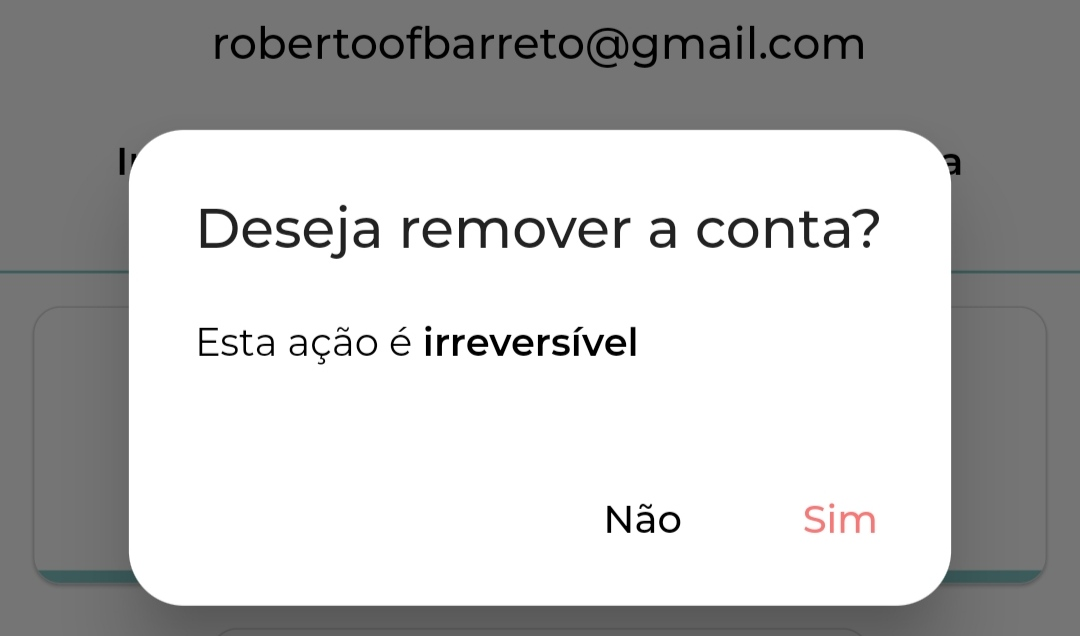
\includegraphics[width=0.4\textwidth]{images/implementacao/frontend/gestao_users/1686054218255.jpg} }}%
 \label{fig:70}%
\end{figure}

Sempre que um utilizador sem acesso ou com a conta apagada efetua o \textit{login}, receberá uma mensagem de erro que menciona que não possui acesso à conta impedindo a continuação do processo.

\begin{figure}[htb]
 \centering
 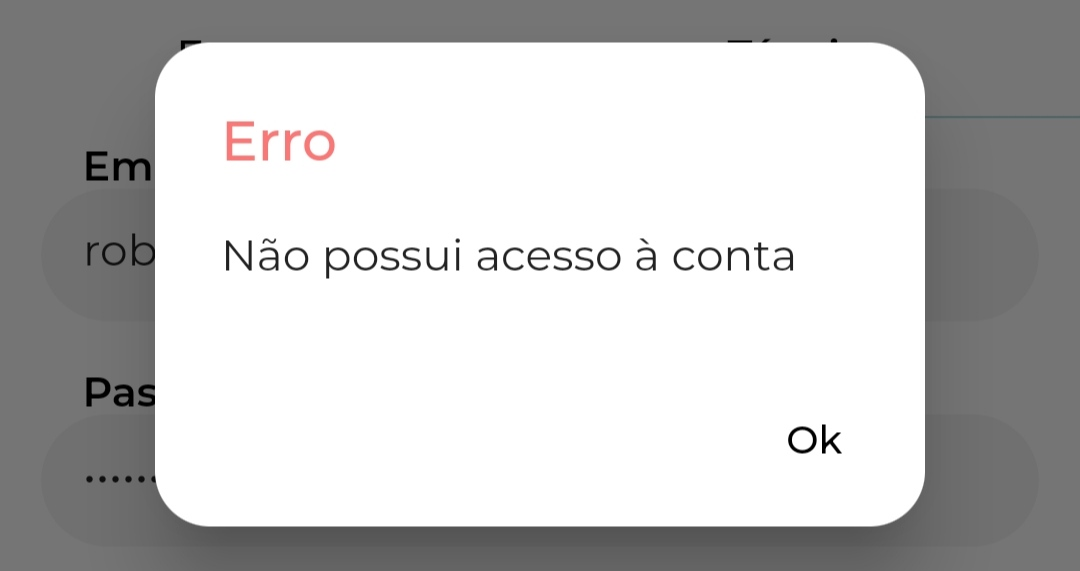
\includegraphics[width=0.4\textwidth]{images/implementacao/frontend/gestao_users/1686054218243.jpg}
 \caption{Aviso de login a conta sem acesso}
 \label{fig:71}
\end{figure}